\noindent\begin{figure}[htb]
\centering
\begin{minipage}[t]{0.48\textwidth}
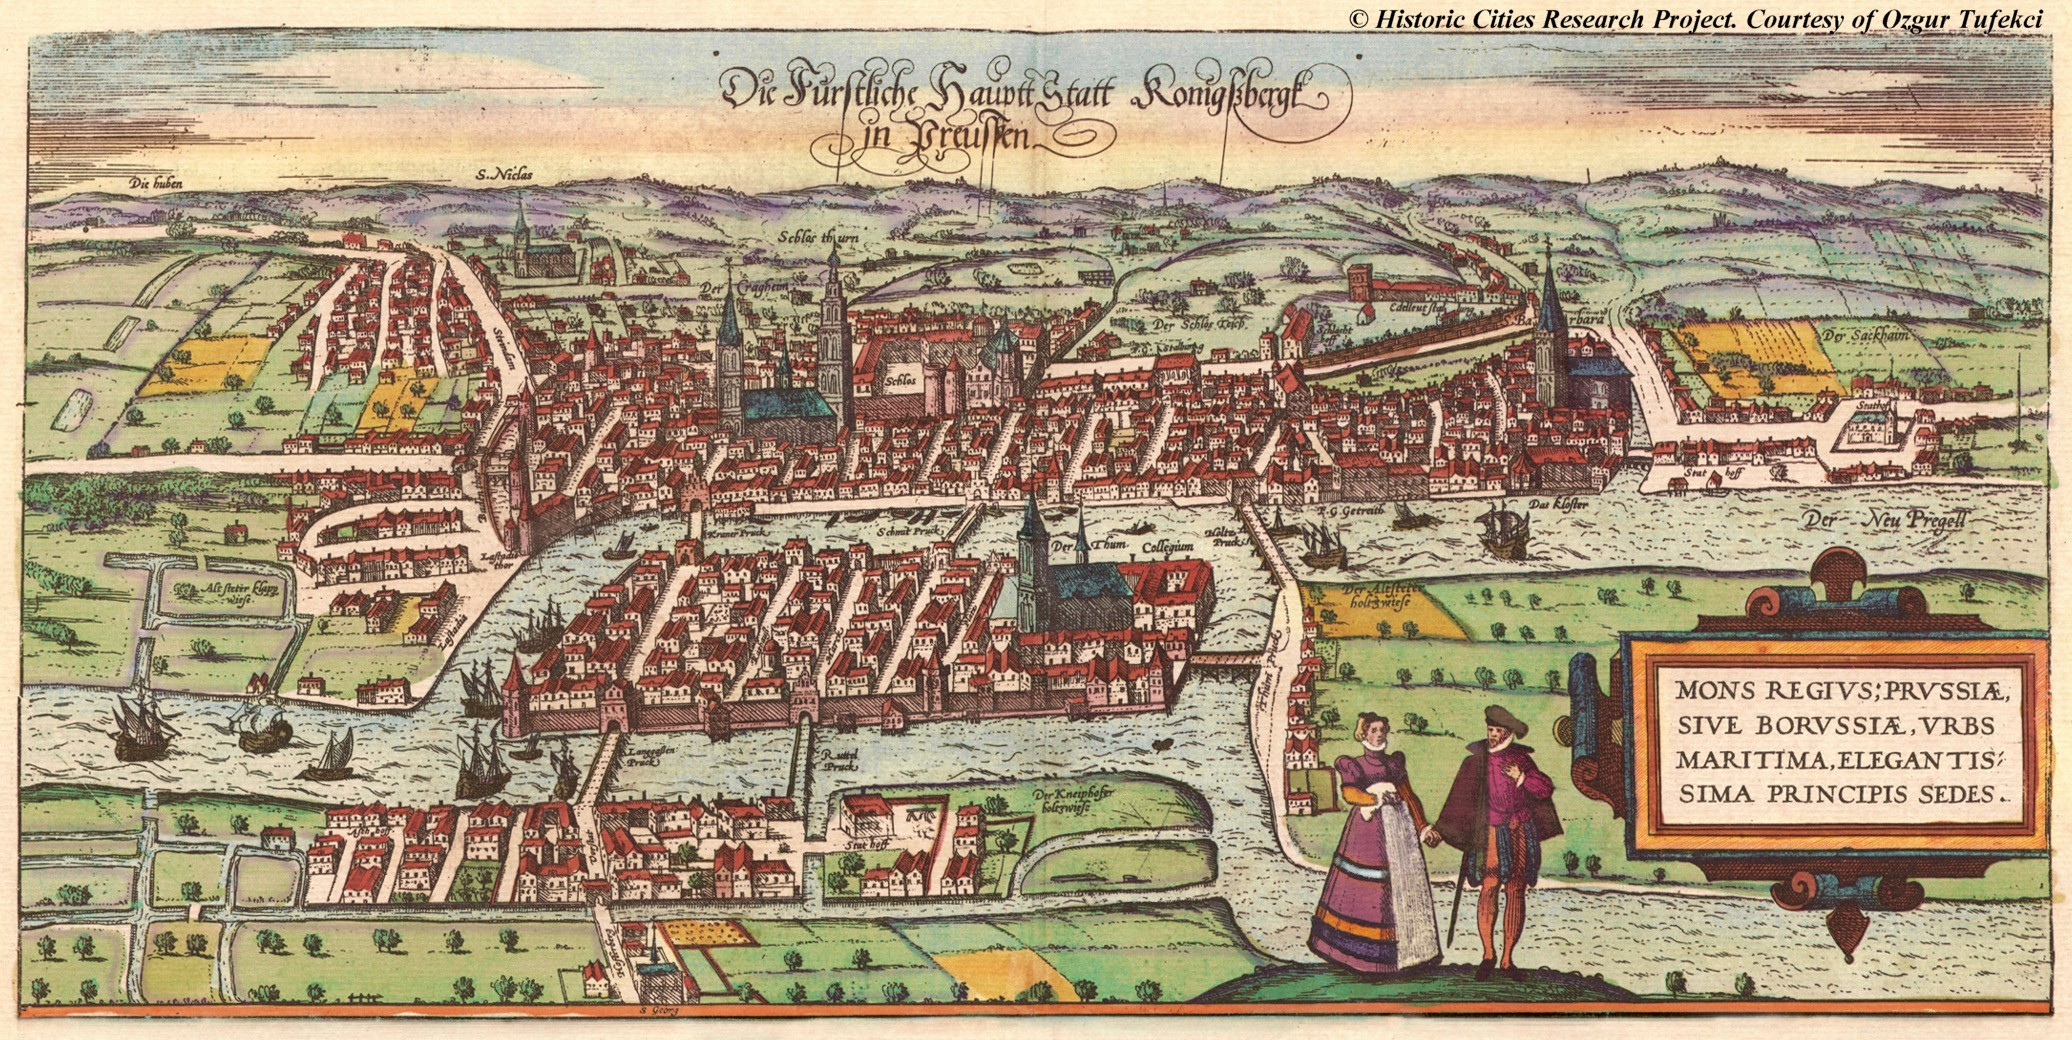
\includegraphics[width=1\textwidth]{images/konigsberg.jpg}
\end{minipage}\begin{minipage}[b]{0.48\textwidth}
\centering
\begin{tikzpicture}
    \tikzset{LabelStyle/.style= {draw}}
    \GraphInit[vstyle=Normal]
    \node[VertexStyle](A){a};
    \node[VertexStyle,right=of A](B){b};
    \node[VertexStyle,right=of B](C){c};
    \node[VertexStyle,above= 1.2cm of B](D){d};
    \draw[EdgeStyle](B) to node[LabelStyle]{} (D);
    \tikzset{EdgeStyle/.append style = {bend left}}
    \draw[EdgeStyle](A) to node[LabelStyle]{} (B);
    \draw[EdgeStyle](B) to node[LabelStyle]{} (A);
    \draw[EdgeStyle](B) to node[LabelStyle]{} (C);
    \draw[EdgeStyle](C) to node[LabelStyle]{} (B);
    \draw[EdgeStyle](A) to node[LabelStyle]{} (D);
    \draw[EdgeStyle](D) to node[LabelStyle]{} (C);
\end{tikzpicture}
\end{minipage}
\caption*{\textsf{The city of K{\"o}nigsberg in an old postcard with its graph-theoretical representation, where the bridges are the edges of the graph and the city parts are represented by nodes. This city inspired Euler to start graph theory.}}
\end{figure}

%%%%%%%%% INTRO GENERALE COMPLEX NETWORKS
\section{Complex networks science and the brain}
The brain is an extremely complex organ, whose dynamics is driven by the internal activity of its constituents, the neurons, responding adaptively to an ever-changing outside environment.
The elements of the nervous system interact and react over the organic substrate that they themselves define, and shape an extremely intricate pattern of electrical and metabolic activities, giving rise to the outstanding set of abilities and possibilities typical of most evolved organisms.
Nonetheless, the notion that brain function can be reduced to the single operations of its constituents is as flawed as its complementary idea that cognition can be understood without making reference to its biological substrate.
Instead, what science is increasingly recognizing is that for most systems in nature, in order to conserve the properties under investigation, it is necessary to remain within a certain level of complexity and to contemplate the multiple interactions of simple subsystems taken as a whole. It is known, in fact that many systems, despite radically different at their microscopic level, share many remarkable organizational properties, when analyzed in their entirety.

A window over the formidable and irreducible complexity of the brain can thus be opened by specific theoretical tools able to account for the brain multi-scale organization, its hierarchical structure and its modular composition.

The study of brain connectivity has already made possible many advances in specializations of neuroscience, from the identification and structural characterization of the cytoarchitecture, to the macro-scale connectivity at level of nerve fibers.
Specifically, the analysis of the architecture of the nervous is based on the idea that the brain can be thought as a complex system at different spatial and time scales. In this respect, the tools of network theory are the method of election in the analysis of complex systems.
% Such representation relies upon the treatment of the brain as a graph, whose nodes are indicative of particular brain regions and whose lins
%%%%%%
\bigbreak

The methods of network theory date back to the problem of K{\"o}nigsberg bridges, in 1735, when the famous mathematician Leonhard Euler was faced with the problem of finding a path through the city that would cross all the seven bridges just once.
Since then a large amount of knowledge has been accumulated on networks, in what is nowadays known as graph-theory.

In totally general settings, simple graphs are usually defined as a set of nodes, entities representative of some object, connected by a set of links, denoting the strength of the relation between pairs of nodes.
Graphs can be used to represent any type of relation between interacting elements and the idea that graph-theory can be applied to brain networks has been pioneered starting from the middle nineties of the twentieth century, defining a new specialization of systems biology, dubbed ``network-neuroscience''.

In the framework of network neuroscience the modeling of brain in terms of graphs starts from the definition of its nodes. These can be defined as electroencephalography or multi-array electrodes or as anatomically defined regions of histological, MRI or diffusion tensor imaging data. A clear delineation of network nodes, is one of the first steps in the whole pipeline of the graph-theoretical analyses and is highly important for the subsequent statistics that result from the data.

The second step in the definition of a brain network is an estimate of the continuous association between nodes. The links indeed measure the interregional coordination or similarity between nodes.
To be more specific in the case of fMRI studies of resting state functional connectivity, link weights are defined as interregional temporal correlations in the fluctuations of the BOLD signals, and the resulting graph can be represented by an adjacency matrix where the strongest correlations indicate the presence of a link between any two specific areas.
In other applications like Diffusion Tensor Imaging, a technique that is able to show the effective directions of nervous fibers traits in the brain, one can see the links as directly proportional to the number of white matter tracts connecting any two regions.
Additionally, brain networks have also been defined on the basis of inter-subject anatomical covariance~\cite{Evans2013,he2007}, co-activation of different brain regions across individuals subjected to experimental tasks~\cite{crossley2013a}, pharmacological challenges~\cite{Schwarz2007,schwarz2008} or  spectral coherence of EEG electrical time-courses.
All of these networks are ``weighted'' by definition, i.e. their links are associated with real numbers representing a measure of the strength of pairwise interactions between nodes.

The ascendancy of the network neuroscience in the last decade, is driven by the evidence that almost independently from how the networks links are defined, brain networks some common tracts at many spatial and temporal scales.

Among these findings we can mention for example, that they exhibit the \emph{small-world}~\cite{Watts1998,sporns2002} property, in other words, most nodes in a graph can be reached from any other node in just a few hops. Small-worldness in brain networks~\cite{vandenheuvel2008} has been found to positively correlate with higher IQ in humans~\cite{vandenheuvel2009}, suggesting that human intellectual performance is likely to be related to how efficiently our brain integrates information between multiple brain regions.

Additionally, other measures have been correlated with phenotypic and structural traits. ``Rich-clubs'' are subset of high degree nodes who are very \emph{rich} in connections and form a communication backbone that might be valuable in supporting high-level and more cognitively advanced forms of information processing. Interestingly, it's thought that the presence of a rich club increases the diversity of the functional repertoire over and above the effects produced by scale free type topology alone~\cite{senden2014}.
Forms of rich-club organization has been observed in cats, macaque and humans~\cite{vandenheuvel2011,harriger2012,DeReus2013a,collin2014}, comprising portions of prefrontal, parietal, temporal and insular cortex. Rich club nodes and edges participate in a large number of short paths across the network, contributing disproportionately to global communication. 
Abnormal rich-club connectivity is hypothesized to be related  to familial vulnerability for schizophrenia~\cite{collin2014impaired}.

%% FIGURA BULLMORE
\begin{figure}[htb!]
\centering
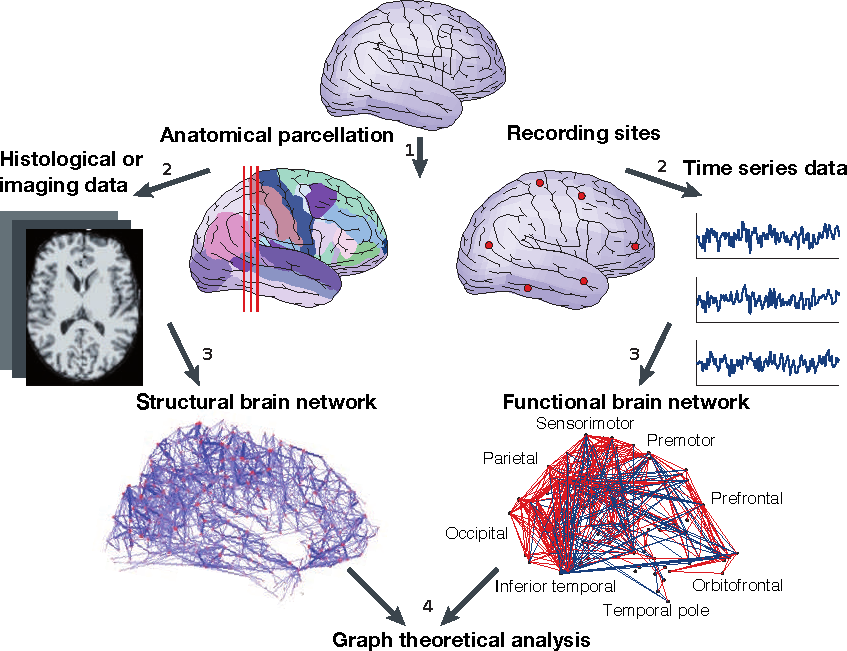
\includegraphics[width=1.0\textwidth]{images/bullmore_2009_pipeline.pdf}
\caption{Structural and functional brain networks can be explored using graph theory through four steps.}
\end{figure}

\bigbreak
Across the many properties that graphs exhibit and that are arguments of further analysis \emph{per se}, one of the most directly observable is that, nodes group together forming some kind of \emph{clusters}.
At this level of meso-scale organization, the topological properties of nodes are more dependent on their neighborhood than on the rest of the graph. When the mesoscopic structure tends to group nodes with similar properties, the meso-scale structure is called \emph{assortative}. Such graphs with assortative structures consist in tightly connected groups of nodes that are themselves loosely connected with other groups. These groups are therefore dubbed as \emph{communities}. 

The organization into communities is one of the most studied properties of networks and a large amount of literature has grown on community detection, as proven by the large review of Fortunato~\cite{fortunato2010}.
The problem of detecting the communities, or ``graph-partitioning'' in the computer-science jargon, is of big theoretical and practical importance.
From the theoretic point of view, communities in networks are representative of the generative probabilistic model underlying the formation of links~\cite{Karrer2011} and tell much about the statistical properties of the networks.
On the other side, practical applications of community detection are fundamental in sociology, computer science, biology and many other fields.

It's being increasingly understood indeed, that like many other information processing systems, the brain exhibit a modular architecture.
Within the modules the information is processed locally and is then shared between modules on a communication backbone~\cite{DeReus2013a,VandenHeuvel2013a}.

Additionally, the modular organization is exhibited hierarchically at different scales, with modules inside modules, a construction that is thought to confer robustness and adaptability to the network~\cite{meunier2010}. This kind of structure implies that modules of heterogeneous size are present at the same time in the brain networks and that an efficient method to detect the presence of large and small modules at the same time together is in order.

Several methods have been proposed to resolve the community structure of complex networks~\cite{fortunato2010,lancichinetti2009}.
Many of these methods involve the definition of a quality function that assigns positive or negative scores to edges connecting nodes within or outside the same community, and heuristics to find the optimal partition of the network that maximize this fitness function. The most popular approach is Newman's ``Modularity maximization'' and variations thereof~\cite{newman2006}.
Following the first demonstration by~\cite{schwarz2008}, partitioning of brain networks using Modularity has been widely applied to assess the brain modular structure.
A few, large modules, including the Default Mode Network, the central network, occipital and frontoparietal networks have been observed with remarkable consistency across subjects and studies~\cite{meunier2010,wang2010}. 

Despite its popularity and merits, Newman’s approach presents some important limitations.
Already at an early stage, Modularity-based methods were shown to suffer from a resolution limit, as they fail to identify modules that are smaller than a scale that depends on the size of the overall network~\cite{fortunato2007}.
As a consequence, even unambiguously defined modules, like complete sub-graphs or cliques, may be unduly merged into larger communities when they are too small compared to the size of the network. Subsequent work by various groups has shown that the resolution limit is quite pervasive~\cite{lancichinetti2009,traag2011,squartini2015,lancichinetti2011,kawamoto2015}, and affects, to a different extent, many other methods, including Reichardt and Bornholdt’s~\cite{reichardt2006}, Arenas and Gomez'~\cite{arenas2008}, Ronhovde and Nussinov's~\cite{ronhovde2009}, Rosvall and Bergstrom's (\emph{Infomap})~\cite{rosvall2008,kawamoto2015} and others.

Fixes have been proposed to circumvent the resolution limit, including the introduction of a tunable parameter that enables analysis of the network at an adjustable resolution level~\cite{reichardt2006,ronhovde2010,yeo2011}. However, this requires prior knowledge of the expected size of the communities for the tuning of the resolution parameter. Moreover, it has been shown that an  adjustable resolution parameter may reduce the tendency to merge small clusters, but only at the cost of unduly splitting large clusters~\cite{lancichinetti2011}. Adjustment of the resolution parameter is an attempt to balance these two biases, but multiresolution methods fail to recover community structures comprising heterogeneous distributions of cluster sizes~\cite{lancichinetti2011}. 

However, real-world networks are characterized by the coexistence of clusters of very different sizes, and no single parameter can adapt to the variety of network topologies observed in nature.
Hence, the resolution limit may represent a critical shortcoming for the study of brain networks and is likely to have affected many of the studies reported in the literature.

%Here, we present only two, from the pletora of examples that take advantage of the application of community detection.
%In sociology, the definition of social cliques is important to identify sets of persons with some social relation~\cite{alba1973}. The social-network LinkedIn, in fact, applies community detection as a recommendation system to suggest new friends to the users.
%Biology is extremely rich of examples where community detection plays an important role. The definition of molecular complexes that take part to the same metabolic pathway and that have the similar functions within the cell is expressed as community detection on the graph of protein-protein interaction.

Before delving into the details of community detection, a short introduction to the methods and the jargon of graph-theory is in order.
In Section~\ref{sec:elementsofgraphtheory} we introduce the mathematical concepts of graph theory. In Section~\ref{sec:communitydetectioninnetworks}, we present the problem of community detection in networks. The Newman's Modularity and the null model upon which its based is discussed in~\ref{sec:newman_modularity}. The bad consequences of Modularity maximization i.e the resolution limit and degeneracy are discussed thoroughly in~\ref{sec:resolutionlimit}, followed by approaches to make the resolution limit less problematic.
%Finally, Surprise, an approach that really mitigates the resolution limit is briefly introduced in section~\ref{sec:surprise}. Different applications of community detection based on Surprise will be then the argument of the next chapters.

%%%%%%%%%%%%%%%%%%%%%%%%%%%%%%%%%%%%%%%%%%%%%%%%%%%%%%%%%%%%%%%%%%%%%%%%%%%%
%%%%%%%%%%%%%%%%%%%%%%% ELEMENTS OF GRAPH THEORY %%%%%%%%%%%%%%%%%%%%%%%%%%%
%%%%%%%%%%%%%%%%%%%%%%%%%%%%%%%%%%%%%%%%%%%%%%%%%%%%%%%%%%%%%%%%%%%%%%%%%%%%
\section{Elements of graph theory}\label{sec:elementsofgraphtheory}
Here we provide to the reader the basic mathematical tools to affront the next chapter. We adopt the typical notation used in other works of the network science field~\cite{newman2010book,Estrada2011}.

A \emph{graph} $G=(V,E)$ is a representation of a set $V$ of $n$ nodes, also called \emph{vertices}, connected by $m$ links (or edges), in a set $E$ (Figure~\ref{fig:simple_unweighted_graph}). When a graph has no multiple links and no self-loops is dubbed \emph{simple graph}.
If multiple links exist between two nodes, the graph is called ``multigraph''. Additionally if a node links itself, the graph is called ``loopy'' graph. Figure~\ref{fig:loopy_multigraph} shows a loopy multigraph. Additionally, when the direction of the links is taken in account, the graph is called \emph{directed}, as shown in Figure~\ref{fig:directedgraph}.

\begin{figure}[htb!]
\centering
	\begin{subfigure}[hb]{0.4\textwidth}\centering
		\includegraphics[width=0.75\textwidth]{standalonetikz/tikz_simple_graph.tikz}
		\caption{}
		\label{fig:simple_unweighted_graph}
	\end{subfigure}
	\begin{subfigure}[hb]{0.4\textwidth}\centering
	\includegraphics[width=0.75\textwidth]{standalonetikz/tikz_weighted_graph.tikz}
	\caption{}
	\label{fig:simple_weighted_graph}
	\end{subfigure}
	\begin{subfigure}[hb]{0.4\textwidth}\centering
	\includegraphics[width=0.75\textwidth]{standalonetikz/tikz_loopy_multigraph.tikz}
	\caption{}
	\label{fig:loopy_multigraph}
	\end{subfigure}
	\begin{subfigure}[hb]{0.4\textwidth}\centering
	\includegraphics[width=0.75\textwidth]{standalonetikz/tikz_directed_graph.tikz}
	\caption{}
	\label{fig:directedgraph}
	\end{subfigure}
	\caption{Classes of graphs. {\textbf (a)} is a simple unweighted undirected graph. {\textbf (b)} is a simple weighted undirected graph, {\textbf (c)} is an unweighted loopy multigraph, {\textbf (d)} is a simple directed graph.}
\end{figure}

The adjacency matrix $\mathbf{A}=\{A_{ij}\} \in \{0,1\}^{n \times n}$ of a binary (undirected) graph is a square $n\times n$ symmetric matrix with elements $A_{ij}=1$ when an edge exists between vertex $i$ and $j$ and $0$ otherwise.

An \emph{edge-weighted graph} (also called weighted graph) $G=(V,E,\omega)$ is a graph that has a set of weights $\omega$ on the links (Figure~\ref{fig:simple_weighted_graph}). Although not true in general, we consider only weighted undirected graphs with symmetrical real adjacency matrix, meaning that if an edge exists between node $i$ and $j$ the weight from $i$ to $j$ is the same as the weight from $j$ to $i$: $\omega_{ij}=\omega_{ji}$. The weighted adjacency matrix,  indicated as $\mathbf{W}=\{ \omega_{ij} \} \in \mathbb{R}^{n\times n}$ is a real, square $n \times n$ symmetric matrix.

The simplest property of the graph, once defined nodes and edges, is the \emph{density} $\rho$. It is defined on a simple graph as the ratio of the number of edges over all possible edges:
\begin{equation}
\rho = \frac{m}{\binom{n}{2}} = \frac{2m}{n(n-1)}.
\end{equation}
A \emph{dense} graph is a graph where almost every possible pair of nodes is connected with an edge. Conversely, a graph is termed \emph{sparse} if the density is low, meaning that also the adjacency matrix is sparse and the number of edges has the order of magnitude of the number nodes $m ~\approx \mathcal{O}(n)$.

The number of edges incident to a node in a simple graph is called \emph{degree}, denoted as $k_i$. Every half edge incident to a node is called \emph{stub}. A vertex with degree $k_i$ has therefore $k_i$ stubs.
On simple weighted graphs, the sum of weights of the edges incident to a vertex $i$ is called \emph{strength} and is denoted as $s_i$. 
In matrix terms, degree and strength are the sums over rows of the adjacency matrix $d_i=s_i=\sum_{j=1}^n A_{ij}$. It must be noted that degree and strength are equal on binary graphs, but different for weighted graphs.

The \emph{degree sequence} $\{k_i\}$ $\forall i=1,\ldots,n$ is the sequence  of the degrees of the vertices, with these numbers put in ascending order, with
repetitions as needed. By the \emph{handshaking lemma}~\cite{leiserson2001}, the sum of all node degrees is equal to twice the number of links:
\begin{equation}
\label{eq:handshaking_lemma}
\sum_{i=1}^n k_i=2 |E|,
\end{equation}
consequently the \emph{average node degree} is given by
\begin{equation}
\left< k \right> = \frac{2m}{n}.
\end{equation}

The \emph{neighborhood} of node $i$ is the set $\Gamma_i=\{j \in V | (i,j) \in E \}$. In other words, the neighbor nodes of $i$ are the nodes which share and endpoint edge to $i$. 
A \emph{path} in a graph is a sequence of edges such that the destination of each edge in the sequence is always the source of the following edge. A \emph{cycle} is a closed path, i.e. a path where the origin and destination nodes are the same.

A graph that has all the possible links, indicated by $K=(V,V\times V)$ is called \emph{complete graph} or \emph{clique} (Figure~\ref{fig:completegraph}). Complete graphs on $n$ nodes, indicated as $K_n$ have a total of $m=\binom{n}{2}$ edges and density equal to $1$.
The complementary graph $\bar{G}$ is the graph that has edges where $G$ has no edges and vice-versa, formally $\bar{G}=(V,V\times V - E)$.
The \emph{empty graph} is therefore defined as the complementary graph of the clique $\bar{K}$, as it has $n$ nodes and no edges (Figure~\ref{fig:emptygraph}). The \emph{cycle graph} $C_n$ is a graph containing a single cycle through all nodes and is the smallest connected cyclic graph (Figure~\ref{fig:cyclegraph}). A \emph{tree graph} is a graph with no cycles and exactly $n-1$ edges.

\begin{figure}[htb]
\centering
	\begin{subfigure}[t]{0.3\textwidth}\centering
		\begin{tikzpicture}
			\tikzset{LabelStyle/.style= {draw,font = \small}}
			\GraphInit[vstyle=Normal]
			\SetGraphUnit{1.5}
			\begin{scope}[rotate=18]
			\Vertices{circle}{a,b,c,d,e}
			\end{scope}
			\Edges(a,b,a,c,a,d,a,e,b,c,b,d,b,e,c,d,c,e,d,e)
		\end{tikzpicture}
	\caption{{\footnotesize Complete graph $K_5$}}\label{fig:completegraph}
	\end{subfigure}
	\begin{subfigure}[t]{0.3\textwidth}\centering
		\begin{tikzpicture}
		\tikzset{LabelStyle/.style= {draw,font = \small}}
		\GraphInit[vstyle=Normal]
		\SetGraphUnit{1.5}
		\begin{scope}[rotate=18]
		\Vertices{circle}{a,b,c,d,e}
		\end{scope}
		\end{tikzpicture}
	\caption{{\footnotesize Empty graph $\bar{K}_5$}}\label{fig:emptygraph}
	\end{subfigure}
	\begin{subfigure}[t]{0.3\textwidth}\centering
		\begin{tikzpicture}
		\tikzset{LabelStyle/.style= {draw, font = \small}}
		\GraphInit[vstyle=Normal]
		\SetGraphUnit{1.5}
		\begin{scope}[rotate=18]
		\Vertices{circle}{a,b,c,d,e}
		\end{scope}
		\Edges(a,b,b,c,c,d,d,e,e,a)
	\end{tikzpicture}
	\caption{{\footnotesize Cycle graph $C_5$}}\label{fig:cyclegraph}
	\end{subfigure}
\end{figure}

A subgraph $\mathcal{G}$ of a graph $G$ is said to be \emph{induced} if, for any pair of vertices $i$ and $j$ of $\mathcal{G}$, the pair $(i,j)$ is an edge of $\mathcal{G}$ if and only if $(i,j)$ is also an edge of $G$. In other words, $\mathcal{G}$ is an induced subgraph of $G$ if it has the most edges that appear in $G$ over the same vertex set. If $\mathcal{G}$ is chosen based on a vertex subset $S$ of $V(G)$, then $\mathcal{G}$ can be written as $G[S]$ and is said to be induced by $S$.

A simple graph is said \emph{connected} if there exist a path between any pair of nodes. If the graph itself is not connected, then it is formed by a set of connected subgraphs, also called \emph{weakly connected components}.

%%%%%%%%%%%%%%%%%%%%%%%%%%%%%%%%%%%%%%%%
\subsection{Clustering}\label{sec:clustering}
Grouping nodes according to some criterion is the basis of community detection. 
A set of mutually disjoint, induced subgraphs that covers all the nodes is called a \emph{clustering}.
A clustering $\zeta = \{\zeta_c\}$ of $G$ is a partitioning of the set $V$ into $C$ disjoint sets of nodes, $\zeta_c \subseteq V$, which we call \emph{modules} or \emph{communities}, interchangeably. 
Each module is a node-induced subgraph $\mathcal{G}:=(V[\zeta_c],E[\zeta_c])$, also indicated as $G[\zeta_c]$.

We denote the number of nodes of the module $G[\zeta_c]$ with $n_c$, the number of edges with $m_c$ and the total number of pairs of nodes with $p_c=\binom{n_c}{2}$.

From the notational point of view, a clustering can alternatively be defined with a \emph{node assignment vector} $\sigma \in \mathbb{N}^n$ in which every node is assigned to an integer label representing the community index. 

The \emph{Kronecker delta} on the assignment vector $\delta(\sigma_i,\sigma_j)=1$ indicates when two nodes lie in the same module and $\delta(\sigma_i,\sigma_j)=0$ when they belongs to different modules.

The \emph{internal degree} $k_{\textrm{int}}(i)$ of vertex $i$ in the module $\mathcal{G}$ is the number of edges connecting $i$ to other vertices in $\mathcal{G}$. If $k_{\textrm{ext}}(i)=0$, the vertex has neighbors only within $\mathcal{G}$, on the other hand if $k_{\textrm{int}}(i)=0$, the vertex is disjoint from $\mathcal{G}$ and should not be part of the same community.

The \emph{external} degree $k_{\textrm{ext}}(i)$ of vertex $i$ in the module $\mathcal{G}$ is the number of edges connecting $i$ to vertices not in $\mathcal{G}$.

The \emph{subgraph internal degree} $K_{\textrm{int}}(\mathcal{G})$ is the sum of the internal degrees of its vertices.
Likewise, the \emph{subgraph external degree} $K_{\textrm{ext}}(\mathcal{G})$ is the sum of the external degrees of its vertices.
The \emph{subgraph total degree} $k(\mathcal{G})$ is the sum of the degrees of the vertices of $\mathcal{G}$. By definition, $K(\mathcal{G}) = K_{\textrm{ext}}(\mathcal{G}) + K_{\textrm{int}}(\mathcal{G})$. For convenience of notation we will denote without loss of generality $K_{\textrm{int}}(\mathcal{G}[ \zeta_c ])$ as $K_c$, specifying the full notation where is needed.

\begin{figure}[htb]\centering
\begin{tikzpicture}
	\GraphInit[vstyle=Normal]
	\SetGraphUnit{1.5}
	\Vertices{circle}{a,b,c,d,e}
	\Edge[label=1](a)(b)
	\Edge[label=2](a)(c)
	\Edge[label=0.5,style={pos=0.25}](a)(d)
	\Edge[label=3](a)(e)
	\Edge[label=1](c)(b)
	\node[draw=black!50,dashed,rounded corners=5mm,fit=(b.north) (a.south) (c.west) (a.east)](BORD) {};
	\node[left of=BORD,anchor=east, inner sep=1cm]{$\mathcal{G}$};
\end{tikzpicture}
\caption{Internal degree $k_{\textrm{int}}(a)=2$, internal strength $s_{\textrm{\textrm{int}}}(a)=3$, external degree $k_{\textrm{ext}}(a)=2$, external strenght $s_{\textrm{ext}}(a)=3.5$.}
\label{fig:internaldegree}
\end{figure}

The \emph{intracluster density} of the subgraph $\mathcal{G}$ is defined as the ratio of the intracommunity edges over the number of pairs 
\begin{equation}
\rho_{\textrm{int}}(G)=\frac{m_c}{p_c} = \frac{2 m_c}{n_c(n_c-1)}.
\end{equation}

The \emph{inter-cluster density} is instead defined as the ratio of edges with one endpoint in $\mathcal{G}$ and the other in $G-\mathcal{G}$, over the total possible number of edges connecting $\mathcal{G}$ with the rest of the graph: 

\begin{equation}
\rho_{\textrm{ext}}=\frac{m-m_c}{n_c(n-n_c)}.
\end{equation}

\noindent At level of whole graph partitioning, the previous definitions are easily applied. The total intracluster edges and total intracluster node pairs numbers are the sum over all modules $c$ of intracommunity edges and node pairs:
\begin{align}
&m_\zeta= \sum \limits_{c=1}^C |E[\mathcal{G_c}]| = \sum \limits_{c=1}^C m_c \\
&p_\zeta= \sum \limits_{c=1}^C \binom{|V[\mathcal{G_c}]|}{2} = \sum \limits_{c=1}^C p_c.
\end{align}

\subsubsection{Communities}
Although no definition of community is universally accepted, the majority of community detection methods aim at implicitly or explicitly finding the best trade-off between intra- and inter-cluster density over all the communities.
A tentative definition of theoretically sound and well defined concept of community has been made by Radicchi with the so called \emph{weak and strong criteria}~\cite{radicchi2004}.

For a community $\mathcal{G}$ to be defined in \emph{weak} sense, the sum of all degrees within $\mathcal{G}$ must be larger that the sum of all degrees toward the rest of the network:
\begin{equation}\label{eq:communityweak}
\sum \limits_{i \in V[\mathcal{G}]} k_{\textrm{int}}(i) > \sum \limits_{i \in V[\mathcal{G}]} k_{\textrm{ext}}(i)
\end{equation}
that is, on average a weakly defined community has more internal than external edges.

Strong communities are defined on a more stringent criterion, i.e. that each and every node in $\mathcal{G}$ must have more connections within the community than with the rest of the graph:
\begin{equation}
\forall i \in V[\mathcal{G}] \qquad k_{\textrm{int}}(i) > k_{\textrm{ext}}(i).
\end{equation}

Finding strong communities is more difficult that finding weak communities and most algorithms fail in this job, as most of them have their own concept of community. Nonetheless these two last definitions are almost universally accepted and give a precise idea of the meaning of community. Additionally, the weak criterion of community is the basis of the planted-partition model~\cite{condon2000} and its later modifications~\cite{lancichinetti2008} that we'll encounter in the next sections. As a last observation, in both the weak and strong criteria, communities are always connected subgraphs.

\begin{figure}[htb]
\centering
	\begin{subfigure}[t]{0.48\textwidth}\centering
	\begin{tikzpicture}
		\GraphInit[vstyle=Normal]
		\SetGraphUnit{1.5}
		\begin{scope}[rotate=-135]
		\Vertices{circle}{a,b,c,e}
		\end{scope}
		\NOEA[unit=1.414](e){d}
		\Edges(a,b,e,d,c,e,a,c,b)
		\node[draw,gray!80,dashed,rounded corners=2mm,fit=(a.north) (a.south) (a.west) (b.east)] {};
		\node[draw,gray!80,dashed,rounded corners=2mm,fit=(e.north) (e.south) (e.west) (c.east)] {};
		\node[draw,gray!80,dashed,rounded corners=2mm,fit=(d.north) (d.south) (d.west) (d.east)] {};
	\end{tikzpicture}
	\caption{Unweighted graph}
	\label{fig:loopy_multigraphlusterina}
	\end{subfigure}
	\begin{subfigure}[t]{0.48\textwidth}\centering
		\begin{tikzpicture}
		% This is from http://tex.stackexchange.com/questions/1175/drawing-a-hypergraph
		% it's needed to draw clusterings (or hyperedges)
		\tikzset{LabelStyle/.style= {draw,font = \small}}
		\GraphInit[vstyle=Normal]
		\SetGraphUnit{1.5}
		\begin{scope}[rotate=-135]
		\Vertices{circle}{a,b,c,e}
		\end{scope}
		\NOEA[unit=1.414](e){d}
		\Edge[label=4](a)(b)
		\Edge[label=0.5](d)(e)
		\Edge[label=0.2](d)(c)
		\Edge[label=0.1](c)(b)
		\Edge[label=0.4](e)(a)
		\Edge[label=3](e)(c)
		\Edge[label=6](e)(b)
		\Edge (a)(d)
		\node[draw,gray!80,dashed,rounded corners=2mm,fit=(a.north) (a.south) (a.west) (b.east)] {};
		\node[draw,gray!80,dashed,rounded corners=2mm,fit=(e.north) (e.south) (e.west) (c.east)] {};
		\node[draw,gray!80,dashed,rounded corners=2mm,fit=(d.north) (d.south) (d.west) (d.east)] {};
		% \tikzstyle{cluster} = [fill,opacity=.5,fill opacity=.5,line cap=round, line join=round, line width=50pt]
		% \begin{pgfonlayer}{background}
		% \draw[cluster,color=purple] (a) -- (b) -- (c);
		% \draw[cluster,color=green] (e) -- (d);
		% \end{pgfonlayer}
		\end{tikzpicture}
		\caption{Weighted graph }\label{fig:loopy_multigraphlusteringb}
	\end{subfigure}
	\caption{Clustering for a unweighted and a weighted graph.}
\end{figure}

\subsection{Models of random graphs}\label{sec:models_random_graph}

A large effort of network science is in the description of the generative processes that lead to observed networks. In general a random graph is a model network in which some specific set of parameters take fixed values, but the network is random in other respects.
%In the first part of the twentieth century, mathematicians developed advanced theories of random graphs as they needed to compare the properties of real-world networks against random null hypotheses.
The theory of random graphs studies the intersection between graph theory and probability theory. %A random graph is a probability space $(\Omega,\mathcal{F},\mathcal{P})$, where the sample space $\Omega$ is a nonempty set of graphs, the set of events $\mathcal{F}$ is a collection of subsets of the sample space (usually the power set of $\Omega$), and $\mathcal{P}$ is a function that assigns a probability to each event. It is usual to describe a random graph by a sequence of steps to construct it. Such a sequence is called an \emph{random graph model}.

%Given the unavailability of computer simulations at that time, the simplest model dates back to 1959 and is due to Erd\H{o}s and Rényi~\cite{Erdos1959}. In the Erd\H{o}s-Rényi model (also called $G_{n,m}$ model, the sample space $\Omega$ is the set of all graphs having $n$ nodes and $m$ edges.
One of the simples models is the network generated by selecting exactly $m$ edges from the possible $\binom{n}{2}$ edges and placing them at random. This model is mathematically known as $G(n,m)$ or \emph{Gilbert} random graph. In probabilistic terms, the $G(n,m)$ graph is equivalent to say that the network is sampled choosing uniformly from the set $\Omega$ of $\binom{\binom{n}{2}}{m}$ possible graphs. Strictly speaking, a random graph model is better defined as an ensemble of networks, therefore as a probability distribution $\mathcal{P}(\Omega)$ over the space of all graphs $G$. The Gilbert random graph model is then associated with a probability distribution centered in $\mathcal{P}(G)=1/\Omega$ for graphs with $n$ nodes and exactly $m$ edges, and zero otherwise.

A way more useful random graph model is instead due to Erd\H{o}s and Rényi~\cite{Erdos1959}. Some properties of the $G(n,m)$ models are easy to compute, like the mean number of edges, but instead others are more complicated. To solve the analytical computation problems on the $G(n,m)$ model, Erd\H{o}s and Rényi introduced instead a parameter $p_{ER}$ that specifies the probability of an edge to exist given two nodes, rather than picking exactly $m$ edges. Technically the $G(n,p)$ random graph model or \emph{Erd\H{o}s and Rényi} (ER) model, is the ensemble of simple graphs with $n$ nodes in which each simple graph $G$ of $m$ edges appears with probability
\begin{equation}
P(G)={p}_{ER}^{m}(1-p_{ER})^{\binom{n}{2}-m}
\end{equation}
Because of the Bernoulli distribution of edges, this graph model is also called \emph{Bernoulli random graph} or \emph{Poissonian random graph} and generally intended as \emph{the} random graph.

Both the ER and Gilbert models should not show any modular structure as every substructure that appears is effect of random fluctuations due to finite sampling effects.
%We will see, though, in the following chapters that still some algorithms find communities in ER graphs.
As every graph obtained from the Erd\H{o}s-Rényi model is a sample from the the probability space $\mathcal{G}$, is better to talk in term of ensemble averages. In the ER model, the expected number of edges in such a graph is the average over $\binom{n}{2}$ independent coin tosses with probability $p_{ER}$:
\begin{equation}
\left< m  \right> = \binom{n}{2}p_{ER}
\end{equation}
and the expected degree $\left< k \right>$ is the same for every node
\begin{equation}
\left< k \right> = p_{ER}(n-1).
\end{equation}
The probability that a node $i$, chosen at random, has degree $k$ is called the \emph{degree distribution}. In general terms, such probability is expressed as:
\begin{equation}
\Pr(k) = \frac{\left< |\{ i \| k_i=k \}| \right>}{n}.
\end{equation}
In the ER model, a given node is connected with probability $p_{ER}$ to each of the other $n-1$ nodes. Thus, the probability of being connected to a particular $k$ other vertices and not to any of the others is $p^k(1-p)^{n-1-k}$, but since there are $\binom{n-1}{k}$ ways to choose those $k$ other nodes, hence the total probability of being connected to exactly $k$ others is:
\begin{equation}
\Pr(k) = \binom{n-1}{k}p_{ER}^k(1-p_{ER})^{n-1-k}
\end{equation}
a binomial distribution that can be approximated to a Poisson distribution for large $n$:
\begin{equation}
\Pr(k) \approx \frac{(n p_{ER})^k e^{-n p_{ER}} }{k!}.
\end{equation}
\bigbreak
In generalizing the concepts of random networks models, one can define every simple graph on $n$ nodes as the output of a random process where each edge $(i,j) $ is sampled with a probability $\Pr(i,j,{\boldsymbol \theta})$ with $\boldsymbol \theta$ is a vector of hyperparameters. In the simplest case of the ER graph, this generative model is an uniform probability distribution with $\boldsymbol \theta=p_{ER}$ as every pair of nodes is linked by an edge with constant probability:
\begin{equation}
\Pr(i,j) = p_{ER}.
\end{equation}

The ER model, despite its advantages (it allows to compute almost all network measures analytically) does not realistically represent empirical networks. Its Poissonian degree distribution (Figure~\ref{fig:deg_dist_poisson_er}) is far from the degree distributions seen in most of the real-world networks. In fact, the empirical behavior of the degree distribution of real networks is one of the main reasons why they attracted so much interest from the scientific community.

The world-wide-web, as well as the connectome of the worm \emph{C. Elegans}\footnote{\emph{Caenorbiditis elegans}, a small nematode worm, famous as the first living organism whose connectome has been completely mapped.} and many other examples, show that the degree distribution is not centered around a mean value as predicted by ER model. 

\noindent\begin{figure}
\centering
\begin{minipage}[b]{0.5\textwidth}
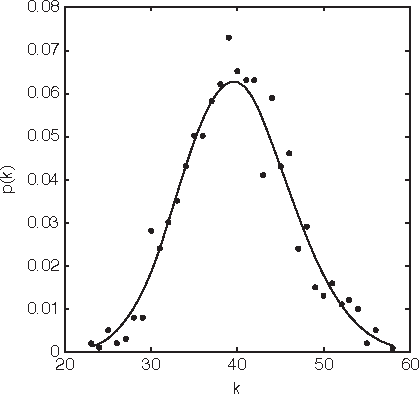
\includegraphics[height=4cm]{images/deg_dist_poisson_er.pdf}
\end{minipage}\noindent
\begin{minipage}[b]{0.5\textwidth}
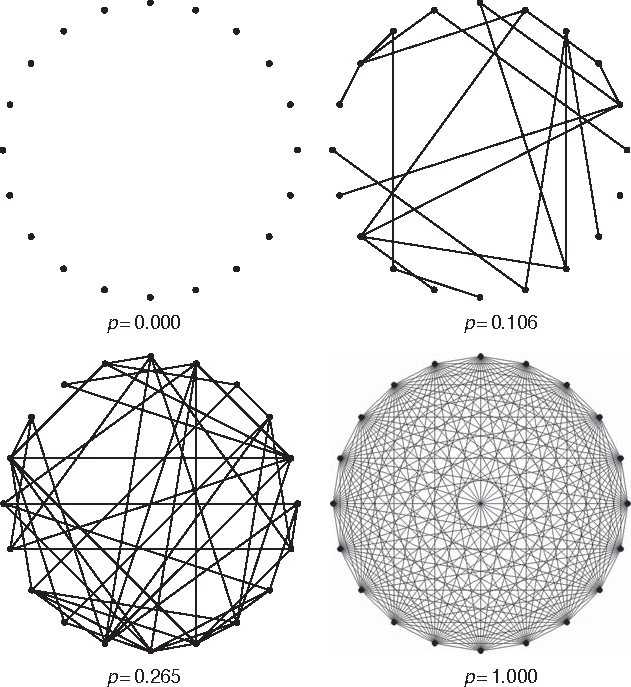
\includegraphics[height=4cm]{images/er_graphs.pdf}
\end{minipage}
\caption{Examples of ER graphs. On the left the Poisson degree distribution of an ER network, $n=1000$,$p=0.04$. On the right ER model instances at different values of $p$. Adapted from~\cite{Estrada2011}.}
\label{fig:deg_dist_poisson_er}
\end{figure}

Instead, in real networks, highly connected nodes exist within a bulk of low connected nodes and the tails of the distribution are not decaying exponentially, producing the observed phenomenon of \emph{heavy tails}.
It turns out, that many networks display a degree distribution that follows a \emph{power-law} form
\begin{equation}
\Pr(k) \propto k^{-\gamma}
\end{equation}
where $\gamma$ is usually included in the $[2,3]$ interval.
Power-law distributions, are also dubbed \emph{scale-free}, as they lack a specific scale. For some multiplicative constant $\alpha$ one indeed has that $P(\alpha k)=f(\alpha)P(k)$ where $f$ is a function only of the parameter $\alpha$. Therefore, the functional form of the power-law remain unchanged.

Hence, in understanding the limitation of the Erd\H{o}s-Rényi model, researchers developed a multitude of generative models of graphs that tried to better model properties like the heavy-tails seen in power-laws or also the \emph{small-worldness} phenomenon, i.e. the observation that most nodes in a network are reachable from every other in a small number of hops.
To keep in account the features of empirical networks, other models of networks have been developed like the models of Watts-Strogatz~\cite{Watts1998} model and Barabasi-Albert~\cite{Barabasi1999}.

For example, in the Watts-Strogatz model a graph with groups of densely connected nodes is generated as follows:
\begin{enumerate}
\item Construct a ring with $n$ nodes and connect each node to the $l$ nearest nodes ($l/2$ in each side of the ring).
\item Choose a node $i$ and the edge $e$ that connects $i$ to its nearest neighbor in a clockwise manner.
\item With probability $p_r$ replace the edge $e$ by the edge that connects $i$ to a node taken at random according to an uniform distribution over the entire ring.
\item Repeat the steps 2 and 3 for each node in clockwise manner.
\item Choose a node $i$ and the edge $e$ that connects $i$ to its second neighbor in a clockwise sense and repeat the steps 2-4.
\item Repeat the process considering the third nearest neighbor and so on, until each edge of the original lattice has been considered.
\end{enumerate}

The resulting graph shows the property of having short average path length, although the degree distribution is not power-law.
To prevent this issue, the Barabasi-Albert graph model aims to construct graphs with a dynamic attachment process.
In the BA model, one considers a small number $n_0$ of initial nodes. Then at each step, one adds a new node and connect it to a fixed number $(\leq n_0)$ of nodes that already exist in the network. The probability that the new node will be connected to a node $i$ is then proportional to $k_i^{p_s}$,  where $p_s$ is a parameter called the \emph{scaling exponent}. That algorithm generates graphs in which the frequency of nodes with degree $k$ is asymptotically proportional to ${k}^{-3}$. This power relationship between frequencies and degrees indicates that this model accounts for the power-law distribution of degrees seen in many real networks.

Although very well studied, both models are still lacking a strong community structure and more complex models have been studied by the network science community.

\section{Community detection in networks}
\label{sec:communitydetectioninnetworks}

The process of grouping nodes in a graph to establish their common behavioral properties, is a popular technique that goes under the name of \emph{community detection}. As the definition of community is not well stated, it is therefore important to have a quantitative way to evaluate the goodness of a clustering.

A \emph{quality function} is a function $\mathcal{Q}$ that given a clustering of a graph $\zeta$ returns a scalar number. Usually one identifies ``good'' clusterings with high scores of the quality function and ``bad'' clusterings with low scores. In this sense, is possible to rank partitions from bad to good, although is important to stress that the definition of ``good'' or ``bad'' is an \emph{ill-posed problem} as every quality function one designs puts the emphasis on some features of the community organization and perhaps not on others.
Here and in the following sections, we strongly point out that the concept of quality function and community detection methods are separate as the first is a way to assess the goodness of a partition while the second relies on quality function to design efficient algorithms and heuristics to find such good partitions.

One of the most important properties of a quality function is when it can be expressed as sum over communities. Such quality functions are dubbed \emph{additive}: for a generic function of a cluster $f(\zeta_i)$, an additive quality function specify the goodness of a clustering as sum of $f$ over the distinct communities as follows:
\begin{equation}\label{eq:additive_quality}
\mathcal{Q} = \sum \limits_{\zeta_c \in \zeta} f(\zeta_c).
\end{equation}
The majority of quality functions are additive, even if this requirement is not fundamental. In the next section we explore the properties of some of the most important additive quality functions that emerged from the literature of this decade.

\subsection{Spin glass based quality functions}
The simplest requirement of a quality function, is to put emphasis on intracluster edges and penalize intercluster edges. In this terms, local optima should correspond to partitions where the communities emerge as dense areas in the network loosely connected among them.
Here we present a general framework for the definition of suitable quality functions for community detection that meets these requirements.

This framework, introduced by Reichardt and Bornholdt~\cite{reichardt2006} is grounded in statistical mechanics, a branch of physics that studies the macroscopic and microscopic properties of systems of many interacting elements. Within this model, the problem of community detection is cast in terms of finding the \emph{ground state} of a spin glass, a model describing the behavior of large sets of interacting magnets.
Actually, the properties of spin glass models are subject of extremely intensive research in the last decades as their applications range from matter and nuclear physics to neural networks. Here we present only their salient application to community detection and refer the reader to cover the details of the model in other specialized books~\cite{Mezard1990}.

A spin glass model starts from the definition of an Hamiltonian, a multi-variable scalar function that describe the total energy of the physical system with the configuration of its internal components. In our case, the internal components of the system are the nodes. The configuration of the system is then expressed by the community affiliation vector $\boldsymbol\sigma$, meaning that node $i$ stays in the community $\sigma_i$ (see~\ref{sec:clustering}).
The Hamiltonian used by Reichardt and Bornholdt (RB) counts four different contributions. The first two contributions act at intracluster level, positively weighing intracluster edges and negatively weighing intracluster non-edges with coefficients $a_{ij}$ and $b_{ij}$ respectively. The third and fourth contributions work on intercluster edges and non-edges, weighing them with factors $c_{ij}$ and $d_{ij}$. The general form of the RB model is then expressed by the following Hamiltonian:

\begin{align}\label{eq:hamiltonianspinglass}
\mathcal{H}^{\textrm{RB}}(\boldsymbol \sigma) = - \sum_{(i,j)\in V^2} & \left[ a_{ij} A_{ij} - b_{ij}(1-A_{ij}) \right] \delta(\sigma_i,\sigma_j) + \nonumber \\ &  \left[ (c_{ij} A_{ij} - d_{ij}(1-A_{ij}) \right] (1-\delta(\sigma_i,\sigma_j))
\end{align}
with the convention that lowest energy states correspond to best community assignments.
Rearranging Eq.\ref{eq:hamiltonianspinglass} and discarding the terms independent of the partition into a constant $H_0$, one then gets a simpler expression for $\mathcal{H}^{\textrm{RB}}(\sigma)$:

\begin{equation}\label{eq:rbspinglass}
\mathcal{H}^{\textrm{RB}}(\boldsymbol \sigma) = -H_0 - \sum \limits_{(i,j)\in V^2} \left[ \alpha_{ij} A_{ij} - \beta_{ij} \right] \delta(\sigma_i,\sigma_j)
\end{equation}
where the two parameters $\alpha_{ij}=a_{ij}+b_{ij}+c_{ij}+d_{ij}$ and $\beta_{ij}=b_{ij}+d_{ij}$ depend on the \emph{null model} one would like to compare with, i.e. the probability that an edge exists between $i$ and $j$ after random edge rewiring. Hence, a null model provides a mean to compare a specific set of features of a graph, with its randomized version that should specifically lack those features.

It's possible to express any quality function in the form of Eq.~\ref{eq:rbspinglass} as an additive quality function by setting $\alpha_{ij}=1$, $H_0=0$ and moving the summation indexes over the communities rather than over the pairs of nodes, as the sum is only over intracluster edges. The resulting Hamiltonian, expressed here as $\mathcal{H}^{\textrm{RB}}_{\textrm{reduced}}(\sigma)$, then reads:
\begin{equation}\label{eq:rbspinglass2}
\mathcal{H}^{\textrm{RB}}_{\textrm{reduced}}(\sigma) = -\sum_{(i,j) \in V^2} \left[ A_{ij} - \beta_{ij} \right] \delta(\sigma_i,\sigma_j) = - \sum \limits_{c}^C \left[ m_c - \left< m_c \right> \right].
\end{equation}
where $m_c=\sum_{ij}A_{ij}\delta(\sigma_i,c)\delta(c,\sigma_j)$ represents the number of links inside community labeled by $c$ and $\left <m_c \right >=\sum_{ij}\beta_{ij}\delta(\sigma_i,c)\delta(c,\sigma_j)$ is the expected number of links in community $c$ as prescribed by the null model $\beta_{ij}$\footnote{Here and for the rest of the work, we set $P_{ij}:=\beta_{ij}$ for agreement with more conventional notation of null models}. 
Among the additive quality functions that show up in the form of~\ref{eq:rbspinglass2}, the most important and popular is the \emph{Newman-Girvan's Modularity}.

\subsection{Newman-Girvan Modularity}\label{sec:newman_modularity}
Newman-Girvan Modularity (or simply Modularity)~\cite{newman2006}, denoted here and for the rest of the work by $Q^N$, is based on the idea that a network obtained by randomly reshuffling the original graph edges while keeping the same degrees sequence, should not display any community structure. 
An important consequence of such randomization is that any stub in this null model, dubbed ``configuration model'' is equally likely to be connected to any other~\cite{newman2010networks}. Thus, in absence of correlations, the probability that two nodes are connected is expressed by:
\begin{equation}\label{eq:configuration_model}
P_{ij} = \frac{k_i k_j}{2m}
\end{equation}
where $k_i$ and $k_j$ are the degrees of node $i$ and $j$. The ``configuration model''  is of great importance in network science as it assigns higher probability of link to nodes with high degrees, a feature that is compatible with most real world networks. 
We'll address the motivations of the configuration model details in the section~\ref{sec:configuration_model}.

In terms of a spin glass model, Modularity thus measures the deviation from the observed intracluster density with respect to the expected intracluster density specified by the configuration model. Modularity is described in the form of~\ref{eq:rbspinglass2} but normalized by the number of edges in the graph. Modularity is then defined in terms of a normalized Hamiltonian that takes the form described in Eq.~\ref{eq:newmanmodularityspinglass}.
\begin{equation}\label{eq:newmanmodularityspinglass}
Q^N =  \frac{1}{2m} \sum_{ (i,j) \in V^2} \left[ A_{ij} - \frac{k_i k_j}{2m} \right] \delta(\sigma_i,\sigma_j),
\end{equation}
whereby optimal partitions have high values of $Q^N$. As already done in Eq.~\ref{eq:rbspinglass2}, Modularity can alternatively be expressed, as sum over communities of the difference of two terms:
\begin{equation}\label{eq:newmanmodularity}
Q^N = \sum_{c}^{C} \left[ \frac{m_c}{m} - \left( \frac{K_{\textrm{int}}(\mathcal{G}_c)}{2m} \right)^2 \right]
\end{equation}

Modularity takes values in the range $[-0.5,1]$, then a good partition should have $Q^N$ values close to unity, identifying groups with many more internal connections than expected at random. In contrast, a bad partition with $Q^N$ closer to zero should identify groups with no more internal connections than we expect at random.

In the next sections we will challenge this idea and show that this observation leads to false statements about modularity of networks, as a general phenomenon dubbed \emph{resolution limit}, heavily affects any quality function based on comparison with global null models and specifically in the case of Newman's Modularity, hits particularly hard.

\subsection{The configuration model}\label{sec:configuration_model}
A central property of the configuration model is the probability $P_{ij}$ of the occurrence of an edge between two specified vertices $i$ and $j$.
Let's consider anyone of the stubs that emerges from vertex $i$.
What is the probability that this stub is connected by an edge to any of the stubs of vertex $j$?
There are $2m$ stubs in total, or $2m - 1$ excluding the one connected to $i$ that we are currently looking at.
Of those $2m - 1$, exactly $k_j$ of them are attached to vertex $j$.
So, given that any stub in the network is equally likely to be connected to any other, the probability that our particular stub is connected to any of those around vertex $j$ is $k_j/(2m-1)$.
In absence of correlations, the probabilities that any two vertices $i$ and $j$ are connected to each other is given by the sum of the two independent probabilities for vertex $i$ and vertex $j$, defining the null model as:
\begin{equation}\label{eq:configuration_model_probability}
p_{ij} = \Pr \left ( a_{ij} | \{ k \} \right) = \Pr(k_i | \{ k \}) + \Pr(k_j | \{ k \})=\frac{k_i k_j}{2m}
\end{equation}

Although Modularity is most frequently applied to \emph{simple graphs} (see Fig.~\ref{fig:simple_unweighted_graph}), the configuration model implies that the randomization is carried over the space of \emph{loopy multigraphs} (Figure~\ref{fig:loopy_multigraph}).
The rewiring probability considers indeed that the stubs of vertices can be reconnected both to the same source vertex (self-loops) or added to already existing edges (multi-edges).
Consider for example the set of matchings on six stubs that form a triangle graph as illustrated in Figure~\ref{fig:configuration_model_stubs}. The configuration model chooses each distinct edge stubs labeling with equal probability. However, not only the first eight distinct reshuffled labelings are possible under configuration model (Fig.\ref{fig:reshuffle_simple_graphs}) but many other distinct matchings, which produce non-simple networks as shown in Figure~\ref{fig:reshuffle_loopy_multigraphs} where just four of them has been generated. 
In fact, the number of possible rewirings that can be generated under the hypotheses of the configuration model, namely the presence of self-loops and multi-edges, is indicated by $\Omega_{CM}$ and can be computed by means of combinatorial arguments as:
\begin{equation}\label{eq:cm_possible_rewirings}
\Omega_{CM} = \binom{2m}{k_1,\ldots,k_n} = \frac{(2m)!}{\prod_i^n k_i!}.
\end{equation}
For the small triangle graph, this number is already very large: 90 different rewirings are possible!

In practice though, the fraction of edges involved in either self-loops or multi-edges is vanishingly small in the large $n$ limit, and thus we may generally ignore them without much impact. 
Hence, the estimate of the probability of rewiring in Eq.~\ref{eq:configuration_model_probability} is only valid in large, sufficiently sparse graphs with a sufficiently bounded degree sequence.
Under these hypotheses the expected number of edges between two vertices in the space of simple graphs is asymptotically the same as the expectation in the space of stub-labeled loopy multigraphs, i.e. the one previously introduced for the definition of Modularity: $\mathbb{E}_s[a_{ij} |k] \approx k_i k_j /(2m)$, where $s$ denotes the space of simple graphs.

\begin{figure}[htb]\centering
\begin{subfigure}[t]{0.45\textwidth}\centering
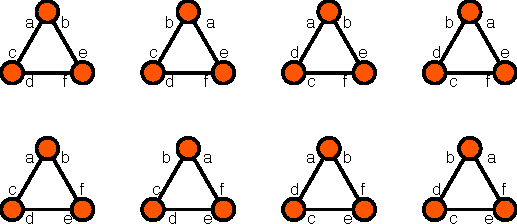
\includegraphics[height=2.5cm]{images/configuration_model_six_stubs.pdf}
\caption{}
\label{fig:reshuffle_simple_graphs}
\end{subfigure}
\begin{subfigure}[t]{0.45\textwidth}\centering
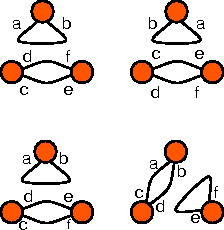
\includegraphics[height=2.5cm]{images/configuration_model_three_stubs.pdf}
\caption{}
\label{fig:reshuffle_loopy_multigraphs}
\end{subfigure}
\caption{Twelve of the ninety different possible rewirings of a triangle graph in the configuration model. In (a) only rewirings leading to simple graphs are considered. In (b) just four rewirings leading to loopy-multigraphs are shown.}
\label{fig:configuration_model_stubs}
\end{figure}
An approach that allows to get the right configuration model depending on the class of graph under exam, relies on the computational simulation of the correct rewiring probability by means of Markov Chain Monte Carlo algorithms, as proposed in~\cite{Fosdick2016}.
In the remaining paragraphs, although flawed, we'll use the classic configuration model from Eq.~\ref{eq:configuration_model_probability} to be adherent to most of the brain networks literature, justified also by the vanishing effects of self-loops in large sparse networks. Nonetheless, we will illustrate many of the problems that the non critical use of Modularity with this null model has introduced.

\subsection{Other null models for Modularity}
Modularity identifies communities as subset of nodes whose internal fraction of edges deviates from the null configuration model on the same subset with the term $m_c/m > (K_c/2m)^2$.
Despite measuring deviation from a null model, Modularity does not take into account the statistical evidence associated with this deviation and as result is not able to separate actual communities from those arising only from statistical fluctuations of the null model. Additionally, Modularity can even find high-scoring partitions in fully random graphs~\cite{Guimera2004} and in artificially built graphs with no community structure~\cite{kehagias2013}.

Importantly, the configuration model is not the only possible null-model to use in spin-glass based quality functions. Different authors proposed several variants of Modularity~\cite{ronhovde2010,ronhovde2009,traag2011} with different null models.
The simplest variation of Modularity is the so-called ER Modularity~\cite{traag2015} that instead of the configuration model uses an Erd\H{o}s-Rényi random graph in which every edge appears with the same probability $p_{ER}$. The number of expected edges $\left< m_c \right>$ in a community of size $n_c$ is thus (in the space of simple graphs):
\begin{equation}
\left< m_c \right> = p_{ER}\binom{n_c}{2}.
\end{equation}
and plugging this null model into the RB model of Eq.~\ref{eq:rbspinglass2} we obtain the model:
\begin{equation}\label{eq:ermodularityrb}
\mathcal{H}^{ER} = -\sum \limits_c^C \left[\frac{m_c}{m}  - p_{ER}\binom{n_c}{2} \right].
\end{equation}
As the most similar ER graph of a given graph is the one that matches its density, the probability parameter $p_{ER}$ must be set equal to the original empirical graph density $\rho$. We therefore obtain the so-called ER Modularity by plugging the graph density in Eq.\ref{eq:ermodularityrb} and inverting its sign, to obtain $Q^{ER}$: 
\begin{equation}
Q^{ER} = \sum \limits_c^C \left[\frac{m_c}{m}  - \rho \binom{n_c}{2} \right].
\end{equation}
Under this model a group of nodes forms a community if its internal density is greater than the graph density $\rho$, on average.
Interestingly, from a machine learning perspective, all spin glass models quantify the discrepancy between observed and expected intramodule fraction of edges by means of a linear loss function.


\section{Resolution limit}\label{sec:resolutionlimit}
Over the years, Modularity attracted a lot of attention as it served as the main tool to inspect whether networks obtained from many different scientific areas, were showing community structure.
The wide use of Modularity has, on one hand, led many researchers to gain interest in complex networks, with results in sociology~\cite{li2008tag}, bioinformatics~\cite{saracc2012topology} and ICT~\cite{java2007we,leskovec2007dynamics} just to mention a few, but on the other hand offered a fallacious view on the community detection problem as an unseen consequence of Modularity maximization was its substantial limit to detect communities smaller than a certain scale.

In 2007, a seminal article by Fortunato and Barthelemy~\cite{fortunato2007} did a thoroughly analysis of Modularity. Their work showed the inability of Modularity to correctly identify communities that are smaller than a certain scale, determined by the square root of the number of edges. They dubbed this general phenomenon \emph{resolution limit}.

To illustrate what is meant by the resolution limit, here we follow the example of Fortunato and Barthelemy, with some obvious notational change.
Let us consider a toy network, $G=(V,E)$ that is composed of three subnetworks, as shown in~\ref{fig:figure_1_barthelemy}A.
The first subnetwork, a subgraph $G_0$ with $n_0$ nodes and $m_0$ edges is connected to two cliques, $G_1$ and $G_2$ by $m_{01}$ and $m_{02}$ links respectively. The two cliques are also connected by a number of $m_{12}$ links as shown in Figure~\ref{fig:figure_1_barthelemy}.

While $G_1$ and $G_2$, are complete subgraphs and are expected to be modules by construction, $G_0$ may consist of many communities. Maximum Modularity partitions then, should identify $G_1$ and $G_2$ as communities, independently from $G_0$.
To be more specific, let the partition where the two cliques are separated be denoted by $A$, with Modularity value $Q_A$. On the other hand, the partition where the two cliques are merged into a single community is denoted by $B$, with Modularity value $Q_B$.
To ease the calculations, we indicate the number of links $m_{12}$ as functions of $m_1$ and $m_2$, such that $m_{12}=a_{1}$, $m_1=a_2 m_2$, $m_{01}=b_1 m_1$ and $m_{02}=b_2 m_2$ with $a_1,a_2,b_1,b_2 \geq 0$.

As Modularity is a sum over the modules, and the module $G_0$ has the same Modularity $Q_0$ in both partitions, we study the difference $\Delta Q = Q_{A} - Q_{B}$ that, after some manipulations, results:
\begin{equation} \label{eq:resolution_limit_delta}
\Delta Q = \frac{2 m a_1 m_1 - (a_1+b_1+2)(a_2+b_2+2)m_1 m_2}{2m^2}
\end{equation}
Specifically, we want to check when $\Delta Q > 0$, i.e. when the partition $A$ has a higher Modularity than partition $B$. This condition is verified as long as
\begin{equation}
m_2 < \frac{2m a_1}{(a_1+b_1+2)(a_2+b_2+2)}.
\end{equation}
In the case where $a_1=a_2=0$, there are no links between $G_1$ and $G_2$ and the condition is satisfied. When instead the two subgraphs are connected ($m_{12} \neq 0$), it happens that at some values of $m_1$ and $m_2$, the partition where the two modules are merged is preferred, i.e. $\Delta Q <0$. This means that when maximizing $Q^N$ on a network, is possible to miss some important structures, if they are too small.
More specifically, if the two modules have the same size and one sets $a_1=a_2=b_1=b_2=1/m$, is easy to check that Eq.~\ref{eq:resolution_limit_delta} is not satisfied if the number of links in the modules $m_c$, is lower than the square root of the total number of links in the network:
\begin{equation}
m_c < \sqrt{\frac{m}{2}}
\end{equation}

To make this example more concrete we studied numerically a toy network where the three subgraphs take a precise form.
For the sake of illustration, we have defined $G_1$ and $G_2$ as two identical cliques of $5$ nodes connected to $G_0$ by a single edge ($m_{01}=m_{02}=1$) and to each other by $m_{12}$ edges.
The module $G_0$ was defined as a clique of variable size with a number of edges ranging from 45 to 2775. We then computed the numerical difference $\Delta Q$ and plotted it as a function of the number of edges $m_0$ in the $G_0$ clique. The onset of the resolution limit occurs for $\Delta Q$ changes sign and becomes negative for increasing values of $m_0$. For $m_{12}=1$, i.e. when the two cliques $G_1$ ad $G_2$ were connected by only one edge (red curve), $Q$ showed this sign inversion for $m_0 \approx 200$ (Figure \ref{fig:figure_1_barthelemy}B).
With increasing number of intercluster edges $m_{12}$, the resolution limit appeared for smaller and smaller values of $m_0$, eventually leading to $\Delta Q$ values that were always negative, i.e. the two cliques $G_1$ and $G_2$ were always merged by Modularity optimization.


\begin{figure}[htb!]
\centering
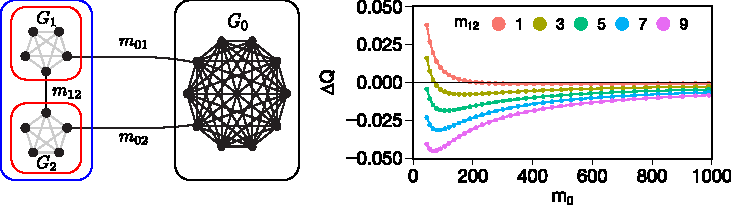
\includegraphics[width=1\textwidth]{images/barthelemy_modularity.pdf}
\caption{Analysis of the onset of the resolution limit for Modularity in a model graph (A) consisting of two cliques, $G_1$ and $G_2$, and a size-varying components $G_0$. The red line indicates the partition $A$, with $G_1$ and $G_2$ as different modules, and the blue line the partition $B$, with $G_1$ and $G_2$ merged into a single module. The graph (B) shows the difference in Modularity for increasing number of edges in $G_0$.}
\label{fig:figure_1_barthelemy}
\end{figure}

An even more striking example of how the resolution limit affects Modularity is when looking at the optimal partition of a synthetic lattice graph, known as ``ring of cliques'', a network made out of identical cliques, connected in a ring-like structure by single links, as shown in Figure~\ref{fig:traag_ring_of_cliques}. 

\begin{figure}[htb!]
\centering
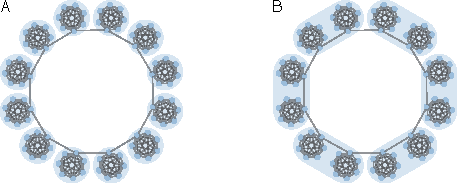
\includegraphics[width=1\textwidth]{images/traag_ring_of_cliques.pdf}
\caption{In this toy network, the intracommunity density is the highest possible, while the intercommunity density is the lowest to keep the network connected. The correct community structure is clearly the one on left (A), but Modularity values is higher for the partition on the right (B), where pairs of cliques are coalesced into separated communities.}
\label{fig:traag_ring_of_cliques}
\end{figure}
If the number of cliques is large enough (they are more than $\sqrt{m}$), Modularity optimization leads to a partition where the cliques are combined into groups of two or more. This phenomenon can be observed already when considering a ring of 30 cliques made of 5 nodes, when the optimal Modularity partition combines cliques in pairs. By extending the number of cliques, then Modularity may merge them in groups of three, fours etc.

In the context of brain networks, the resolution limit first highlighted by Fortunato and Barthelemy may be particularly critical for the analysis of brain connectivity networks, as it may unduly merge modules that are too small, therefore hampering the ability to highlight regions of functional segregation from the rest.

By way of example, certain functional processes, like color vision, have been described as anatomically localized~\cite{zeki1998}, while others, like working memory, have been proposed to involve more globally integrated processing systems~\cite{baddeley2003}.

Hence, we may expect the brain modular structure to comprise heterogeneously distributed communities. Whether the relatively uniform modular structure of brain connectivity, highlighted by Newman's Modularity and other community detection methods in many studies, reflects the true architecture of the brain organization or is the result of the resolution limit is still unclear.

Hierarchical approaches have shown that large modules can be further subdivided, indicating that connectivity networks show structure at different spatial scales~\cite{meunier2009}.
However, these findings do not provide information on the optimal partition of the network, i.e. the optimal cut through the dendrogram representing connectivity at the different scales.
To this end, an optimization method that does not suffer from the resolution limit would be needed.

\subsection{Resolution parameter}
Fixes have been proposed to circumvent the resolution limit, including the introduction of a tunable parameter that enables analysis of the network at an adjustable resolution level~\cite{reichardt2006,ronhovde2010,yeo2011}.

In this sense, the most common tuning to the Modularity quality function is the one that takes in consideration a \emph{resolution parameter}.
From the definition of $Q^N$ is evident that is possible to tune the size of the detected modules by multiplication of the configuration null model by a constant factor $\gamma_{N} \in [0,1]$, resulting in a modified modularity $Q^N(\gamma)$:

\begin{equation}
Q^N(\sigma,\gamma) = \sum_c^C \left[ \frac{m_c}{m} - \gamma \left( \frac{K_c}{2m}\right)^2 \right]
\end{equation}

However, this requires prior knowledge of the expected size of the communities for the tuning of the resolution parameter.
Moreover, it has been shown that an  adjustable resolution parameter may reduce the tendency to merge small clusters, but only at the cost of unduly splitting large clusters. 
Indeed this is due to two opposite coexisting effects: the tendency to merge small subgraphs, which dominates when the resolution is low and the tendency to split large subgraphs, which dominates when the resolution is high.
In benchmark networks with heterogeneous distributions of cluster sizes, the simultaneous elimination of both biases is not possible and multiresolution modularity is not capable to recover the planted community structure even in graphs where the ground-truth structure is evident.
Therefore, adjustment of the resolution parameter is an attempt to balance these two biases, but multiresolution methods fail to recover community structures comprising heterogeneous distributions of cluster sizes~\cite{lancichinetti2011}. 

Real-world networks are characterized by the coexistence of clusters of very different sizes, therefore no single parameter can adapt to the variety of network topologies observed in nature.
Hence, the resolution limit may represent a critical shortcoming for the study of brain networks and is likely to have affected many of the studies reported in the literature.


\subsection{Resolution-limit free quality functions}
Among these models of quality function based on spin glass models, Traag et al~\cite{traag2011} takes as null model a constant quantity specified by a parameter $\gamma_{\textrm{CPM}}$.    

The \emph{Constant Potts Model} (CPM) identifies community as subset of nodes whose internal density $\rho_c$ is bigger than the overall graph density multiplied by a factor $\gamma_{\textrm{CPM}}$ that defines the typical scale of the communities. In the framework of Reichardt and Bornholdt, the CPM model has the following Hamiltonian: 
\begin{equation}\label{eq:cpm_hamiltonian}
H(\sigma)^{\textrm{CPM}} = - \sum \limits_{(i,j) \in V^2} \left[ a_{ij} - \rho \gamma_{\textrm{CPM}} \right] \delta(\sigma_i,\sigma_j).
\end{equation}
A rework of Eq.~\ref{eq:cpm_hamiltonian} permits to write the CPM model as:

\begin{equation}\label{eq:cpm_ermodel}
H(\sigma)^{\textrm{CPM}} = - \sum \limits_c^C \left[m_c - \gamma_{\textrm{CPM}} n_c^2 \right] 
\end{equation}
In other words, the model tries to maximize the number of internal edges while at the same time keeping relatively small communities. The parameter $\gamma_{\textrm{CPM}}$ balances these two imperatives.
In fact, the parameter $\gamma_{\textrm{CPM}}$ acts as the inner and outer edge density threshold.
That is, suppose there is a community c with $m_c$ edges and $n_c$ nodes. Then is better to split it into two communities $r$ and $s$ if: 
\begin{equation}
\frac{m_{r,s}}{2n_r n_s} < \gamma_{\textrm{CPM}}
\end{equation}




%%%%%%%%%%%%%% DEGENERACY %%%%%%%%%%%%%%%%%%%
\section{Degeneracy}\label{sec:degeneracy}
The differences in Modularity between optimal and suboptimal partitions can be very small, as observed in Figure~\ref{fig:figure_1_barthelemy}B, where $\Delta Q$ between the two partitions where the cliques are merged or splitted, remains close to zero for a large range of $m_0$ especially at $m_{12}=1$.
Indeed, even in the case where it would not be beneficial for Modularity to merge two modules, i.e $\Delta Q <0$, this difference can be made arbitrarily close to zero.
As the number of possible different partitions of a graph with $n$ nodes (the Bell number $B_n$) grows faster than exponentially in $n$~\cite{stanley1997}, a combinatorially large number of operations may lead to solutions that are radically different in terms of partition distance, but only slightly suboptimal in terms of modularity, with values very close to the global maximum.
Thus, counterintuitively, when the network becomes more modular, the globally optimal partitions becomes harder to find among the growing number of suboptimal but competitive alternatives.

This consideration explains the observation that nearly-optimal solution tend to group into high-modularity plateaus, although they may differ substantially~\cite{good2009}. This phenomenon, dubbed \emph{degeneracy} affects Newman's Modularity and probably many other spin-glass based quality functions.
As a matter of example, the variation in Modularity for merging a pair of adjacent cliques in the ring of cliques graph shown in Figure~\ref{fig:traag_ring_of_cliques}, is given by:
\begin{equation}\label{eq:modularity_difference_ring_clique}
\Delta Q = \frac{1}{r\left(\binom{n_r}{2}+1\right)}-2r^{-2}
\end{equation}
where $r$ is the number of cliques and $n_r$ the number of nodes in each clique.
In the large $r$ limit, the difference in Eq.~\ref{eq:modularity_difference_ring_clique} tends to a small negative value, indicating that a solution where the cliques are merged, may have a Modularity very close to the optimum. Indeed, already for $r=20$ cliques, $\Delta Q \approx 5\times 10^{-3}$, making all the suboptimal partitions where cliques are merged, very close to the optimal solution.

To make this argument more intuitive, we extrapolated a visually appealing form of the complex landscape of partitions' Modularity for a ring of clique network. We sampled the configuration space of the partitions of a ring of clique network through a Montecarlo procedure and annotated the corresponding values of Modularity for every partition.
We then built a similarity matrix between all sampled partitions and embedded it into a three-dimensional space maintaining similarity relations between partition following a Curvilinear Components Analysis (CCA).
In the embedded manifold, two partitions are close if they are similar and the z-axis encodes the quality function.
An highly degenerate plateu can be observed in~\ref{fig:degeneracylandscape} whereby different solutions with high values of Modularity stay in the same neighborhood.

\begin{figure}[htb!]
\centering
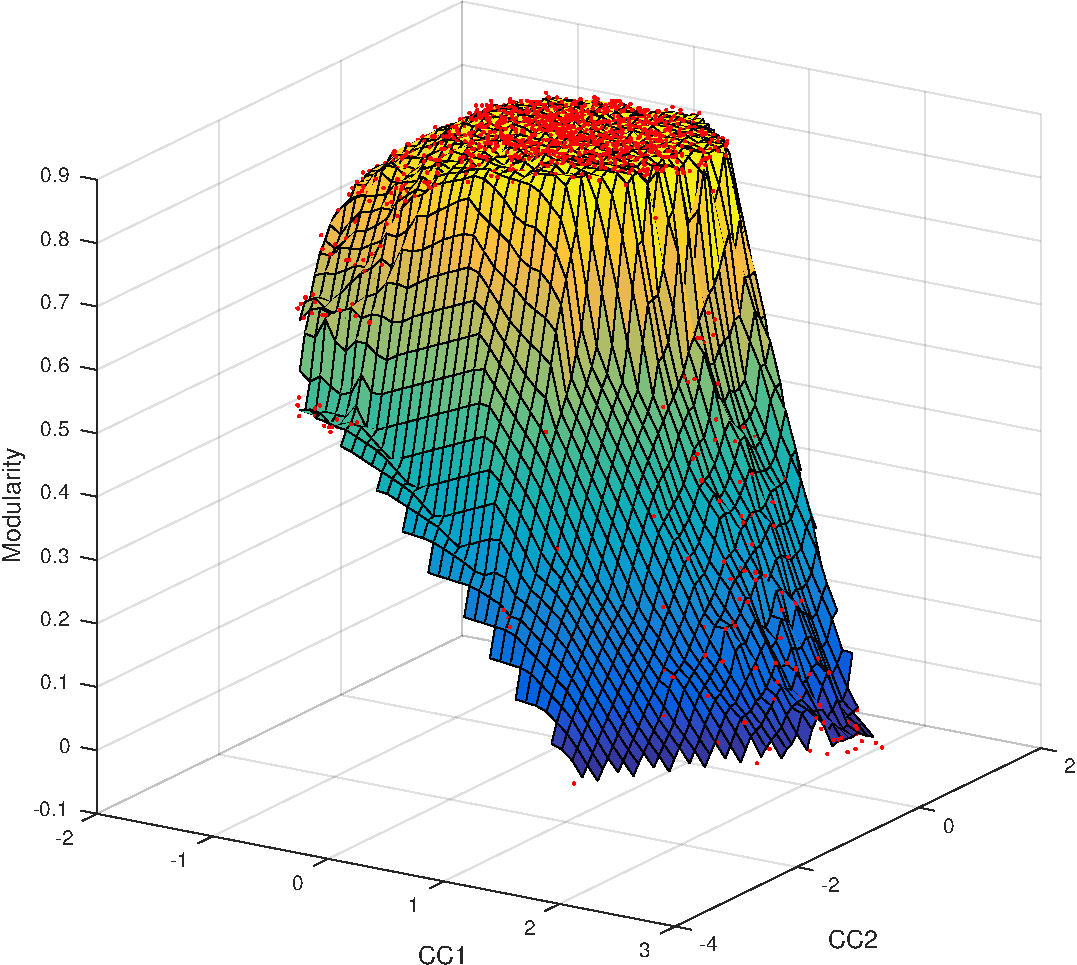
\includegraphics[width=0.6\textwidth]{images/degeneracy_modularity.pdf}
\caption{Degeneracy landscape for Newman's Modularity in a ring of cliques with $r=24$ cliques of $n_r=5$ nodes. The axes CC1 and CC2 are complicated functions of the original partition space computed as to maintain the distance relation between points and their scale is unimportant.}
\label{fig:degeneracylandscape}
\end{figure}

Any quality function suffering degeneracy of solutions, should display an embedded landscape with a plateau of optimal partitions, like the one shown in Figure~\ref{fig:degeneracylandscape}, while instead in the case of the existence of a net global optimum, a sharper peak should be exhibited.